\documentclass[tikz,border=12pt]{standalone}
\usepackage{fontspec}
\newfontfamily\hebrewfont[Script=Hebrew]{Noto Serif Hebrew}
\newcommand{\heb}[1]{{\hebrewfont #1}}
\newfontfamily\igfont[Ligatures=TeX]{Noto Serif}
\newcommand{\igtext}[1]{{\igfont #1}}
\usepackage{amsmath,amssymb}
\usetikzlibrary{positioning,arrows,shapes,fit,calc,backgrounds}
\begin{document}
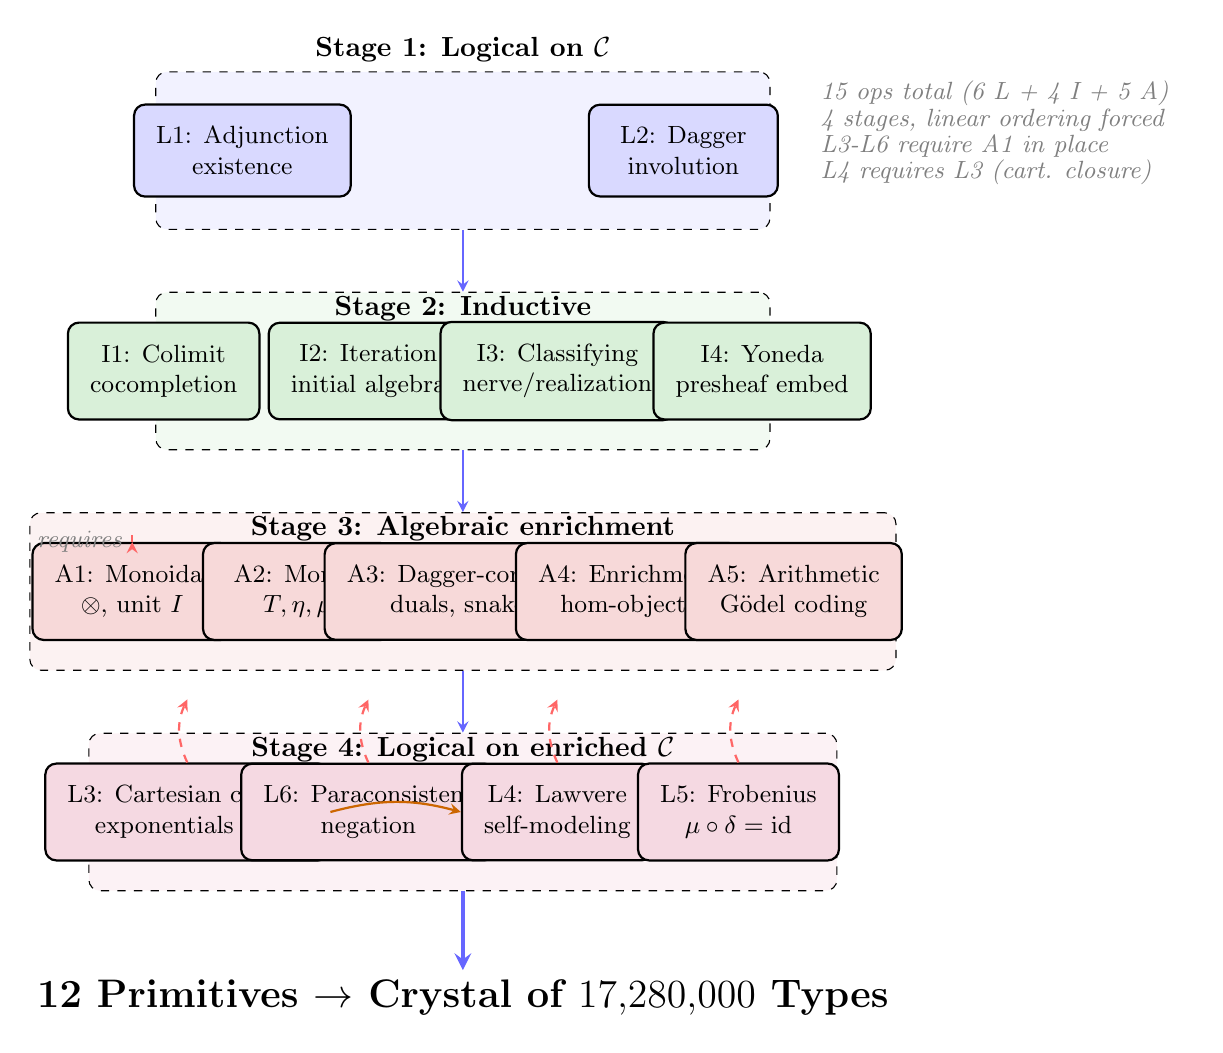
\begin{tikzpicture}[
  opnode/.style={rectangle,draw,thick,rounded corners,fill=#1!15,inner sep=8pt,align=center,minimum width=2.4cm,font=\small},
  dep/.style={->,>=stealth,thick,blue!60},
  stagebg/.style={rectangle,draw,rounded corners,dashed,fill=#1!5,inner sep=8pt},
  precond/.style={->,>=stealth,thick,red!60,dashed,bend left=25},
  lab/.style={font=\footnotesize\itshape,text=gray},
]

% === STAGE 1: Logical on bare category ===
\node[stagebg=blue,minimum width=7.8cm,minimum height=2.0cm] (st1) at (0,0) {};
\node[font=\bfseries,above=0pt of st1] {Stage 1: Logical on $\mathcal{C}$};

\node[opnode=blue] (L1) at (-2.8,0)  {L1: Adjunction\\{\small existence}};
\node[opnode=blue] (L2) at (2.8,0)   {L2: Dagger\\{\small involution}};

% === STAGE 2: Inductive (depends on Stage 1) ===
\node[stagebg=green!60!black,minimum width=7.8cm,minimum height=2.0cm] (st2) at (0,-2.8) {};
\node[font=\bfseries,below=0pt of st2.north,yshift=2pt] {Stage 2: Inductive};

\node[opnode=green!60!black] (I1) at (-3.8,-2.8) {I1: Colimit\\{\small cocompletion}};
\node[opnode=green!60!black] (I2) at (-1.2,-2.8) {I2: Iteration\\{\small initial algebra}};
\node[opnode=green!60!black] (I3) at (1.2,-2.8)  {I3: Classifying\\{\small nerve/realization}};
\node[opnode=green!60!black] (I4) at (3.8,-2.8)  {I4: Yoneda\\{\small presheaf embed}};

\draw[dep] (st1.south) -- (st2.north);

% === STAGE 3: Algebraic (depends on Stage 2) ===
\node[stagebg=red!80!black,minimum width=11cm,minimum height=2.0cm] (st3) at (0,-5.6) {};
\node[font=\bfseries,below=0pt of st3.north,yshift=2pt] {Stage 3: Algebraic enrichment};

\node[opnode=red!80!black] (A1) at (-4.2,-5.6) {A1: Monoidal\\{\small $\otimes$, unit $I$}};
\node[opnode=red!80!black] (A2) at (-2.1,-5.6) {A2: Monad\\{\small $T,\eta,\mu$}};
\node[opnode=red!80!black] (A3) at (0,-5.6)   {A3: Dagger-compact\\{\small duals, snakes}};
\node[opnode=red!80!black] (A4) at (2.1,-5.6) {A4: Enrichment\\{\small hom-objects}};
\node[opnode=red!80!black] (A5) at (4.2,-5.6) {A5: Arithmetic\\{\small G\"odel coding}};

\draw[dep] (st2.south) -- (st3.north);

% Precondition arrows from A1
\draw[precond] (A1.north) to[bend left=25] node[lab,left,pos=0.55] {\small requires} ++(0,0);

% === STAGE 4: Logical on enriched ===
\node[stagebg=purple,minimum width=9.5cm,minimum height=2.0cm] (st4) at (0,-8.4) {};
\node[font=\bfseries,below=0pt of st4.north,yshift=2pt] {Stage 4: Logical on enriched $\mathcal{C}$};

\node[opnode=purple] (L3) at (-3.5,-8.4)  {L3: Cartesian closure\\{\small exponentials $B^A$}};
\node[opnode=purple] (L6) at (-1.2,-8.4)  {L6: Paraconsistent\\{\small negation}};
\node[opnode=purple] (L4) at (1.2,-8.4)   {L4: Lawvere\\{\small self-modeling}};
\node[opnode=purple] (L5) at (3.5,-8.4)   {L5: Frobenius\\{\small $\mu\circ\delta=\text{id}$}};

\draw[dep] (st3.south) -- (st4.north);

% Preconditions (L3, L4, L5, L6 require A1)
\draw[precond] (L3.north) to ++(0,0.8);
\draw[precond] (L4.north) to ++(0,0.8);
\draw[precond] (L5.north) to ++(0,0.8);
\draw[precond] (L6.north) to ++(0,0.8);

% L4 requires L3
\draw[->,>=stealth,thick,orange!80!black,bend left=15] (L3.east) to (L4.west);

% === FINAL OUTPUT ===
\node[below=1.0cm of st4,font=\Large\bfseries] (out) {12 Primitives $\to$ Crystal of $17{,}280{,}000$ Types};
\draw[->,>=stealth,ultra thick,blue!60] (st4.south) -- (out);

% === DEPENDENCY ANNOTATION ===
\node[font=\footnotesize\itshape,text=gray,anchor=north west] at ($(st1.north east)+(0.3,0)$) {\begin{tabular}{l}
\small 15 ops total (6 L + 4 I + 5 A)\\
\small 4 stages, linear ordering forced\\
\small L3-L6 require A1 in place\\
\small L4 requires L3 (cart. closure)
\end{tabular}};

\end{tikzpicture}
\end{document}
